%% Copernicus Publications Manuscript Preparation Template for LaTeX Submissions
%% ---------------------------------
%% This template should be used for copernicus.cls
%% The class file and some style files are bundled in the Copernicus Latex Package which can be downloaded from the different journal webpages.
%% For further assistance please contact the Copernicus Publications at: publications@copernicus.org
%% http://publications.copernicus.org


%% Please use the following documentclass and Journal Abbreviations for Discussion Papers and Final Revised Papers.


%% 2-Column Papers and Discussion Papers
\documentclass[gmd, manuscript]{copernicus}



%% Journal Abbreviations (Please use the same for Discussion Papers and Final Revised Papers)

% Archives Animal Breeding (aab)
% Atmospheric Chemistry and Physics (acp)
% Advances in Geosciences (adgeo)
% Advances in Statistical Climatology, Meteorology and Oceanography (ascmo)
% Annales Geophysicae (angeo)
% ASTRA Proceedings (ap)
% Atmospheric Measurement Techniques (amt)
% Advances in Radio Science (ars)
% Advances in Science and Research (asr)
% Biogeosciences (bg)
% Climate of the Past (cp)
% Drinking Water Engineering and Science (dwes)
% Earth System Dynamics (esd)
% Earth Surface Dynamics (esurf)
% Earth System Science Data (essd)
% Fossil Record (fr)
% Geographica Helvetica (gh)
% Geoscientific Instrumentation, Methods and Data Systems (gi)
% Geoscientific Model Development (gmd)
% Geothermal Energy Science (gtes)
% Hydrology and Earth System Sciences (hess)
% History of Geo- and Space Sciences (hgss)
% Journal of Sensors and Sensor Systems (jsss)
% Mechanical Sciences (ms)
% Natural Hazards and Earth System Sciences (nhess)
% Nonlinear Processes in Geophysics (npg)
% Ocean Science (os)
% Proceedings of the International Association of Hydrological Sciences (piahs)
% Primate Biology (pb)
% Scientific Drilling (sd)
% SOIL (soil)
% Solid Earth (se)
% The Cryosphere (tc)
% Web Ecology (we)
% Wind Energy Science (wes)


%% \usepackage commands included in the copernicus.cls:
%\usepackage[german, english]{babel}
%\usepackage{tabularx}
%\usepackage{cancel}
%\usepackage{multirow}
%\usepackage{supertabular}
%\usepackage{algorithmic}
%\usepackage{algorithm}
%\usepackage{amsthm}
%\usepackage{float}
\usepackage{subcaption}
%\usepackage{subfig}
%\usepackage{rotating}

% Custom commands
\newcommand{\vb}{\mathbf}
\newcommand{\vg}{\boldsymbol}
\newcommand{\mat}{\mathsf}
\newcommand{\diff}[2]{\frac{d #1}{d #2}}
\newcommand{\diffsq}[2]{\frac{d^2 #1}{{d #2}^2}}
\newcommand{\pdiff}[2]{\frac{\partial #1}{\partial #2}}
\newcommand{\pdiffsq}[2]{\frac{\partial^2 #1}{{\partial #2}^2}}

\begin{document}

\title{DCMIP2016, Part 1: Models and Equation Sets}


% \Author[affil]{given_name}{surname}

\Author[1]{Paul A.}{Ullrich}
\Author[2]{Christiane}{Jablonowski}
\Author[3]{James}{Kent}
\Author[4]{Peter}{Lauritzen}
\Author[4]{Ramachandran}{Nair}
\Author[5]{Kevin A.}{Reed}
\Author[4]{Colin}{Zarzycki}

\Author[6]{Thomas}{Dubos}
\Author[7]{Marco}{Giorgetta}
\Author[8]{Elijah}{Goodfriend}
\Author[9]{David A.}{Hall}
\Author[10]{Lucas}{Harris}
\Author[8]{Hans}{Johansen}
\Author[11]{Christian}{K\"uhnlein}
\Author[12]{Vivian}{Lee}
\Author[13]{Thomas}{Melvin}
\Author[14]{Hiroaki}{Miura}
\Author[15]{David}{Randall}
\Author[16]{Alex}{Reinecke}
\Author[4]{William}{Skamarock}
\Author[16]{Kevin}{Viner}
\Author[17]{Robert}{Walko}

\affil[1]{University of California, Davis}
\affil[2]{University of Michigan}
\affil[3]{University of South Wales}
\affil[4]{National Center for Atmospheric Research}
\affil[5]{Stony Brook University}
\affil[6]{Institut Pierre-Simon Laplace (IPSL)}
\affil[7]{Max Planck Institute for Meteorology}
\affil[8]{Lawrence Berkeley National Laboratory}
\affil[9]{University of Colorado, Boulder}
\affil[10]{Geophysical Fluid Dynamics Laboratory}
\affil[11]{European Centre for Medium-Range Weather Forecasting}
\affil[12]{Environment Canada}
\affil[13]{U.K. Met Office}
\affil[14]{University of Tokyo}
\affil[15]{Colorado State University}
\affil[16]{Naval Research Laboratory}
\affil[17]{University of Miami}

%% The [] brackets identify the author with the corresponding affiliation. 1, 2, 3, etc. should be inserted.



\runningtitle{DCMIP2016: Models and Equation Sets}

\runningauthor{Ullrich, et al.}

\correspondence{Paul A. Ullrich (paullrich@ucdavis.edu)}


% User-defined mathematical symbols
\renewcommand{\emph}[1]{{\color{red}\textbf{#1}}}
\newcommand{\pd}[2]{\frac{\partial #1}{\partial #2}}
\newcommand{\p}[1]{\partial #1}
%Then, writing a partial is as simple as $\pd{J}{x}$.
\newcommand{\ol}[1]{{\overline #1}}
\newcommand{\mbf}[1]{{\mathbf #1}}
\newcommand{\mbfol}[1]{\overline{{\mathbf #1}}}
\newcommand{\wdh}[1]{{\widehat #1}}
\newcommand{\wdt}[1]{{\widetilde #1}}
\newcommand{\sss}[1]{{\scriptscriptstyle #1}}
\newcommand{\scs}[1]{{\scriptstyle #1}}

\received{}
\pubdiscuss{} %% only important for two-stage journals
\revised{}
\accepted{}
\published{}

%% These dates will be inserted by Copernicus Publications during the typesetting process.


\firstpage{1}

\maketitle



\begin{abstract}
This paper provides a comprehensive review of the design of modern non-hydrostatic atmospheric dynamical cores, including relevant equation sets, numerical stabilization techniques and idealized physics routines.
\end{abstract}



\introduction  %% \introduction[modified heading if necessary]

{\color{red}INSTRUCTIONS FOR AUTHORS}

{\color{red} Fill in text in section 3, 4, 5, 6, 7 and 8 below.}

\section{Notation}

\subsection{List of Symbols}

Table \ref{tab:symbols} lists the symbols used in this paper.

\begin{table}[h]
\caption{List of symbols used in this manuscript} \label{tab:symbols}
\begin{center}
\begin{tabular}{cl}
\hline Symbol & Description \\ \hline 
$\lambda$ & Longitude (in radians) \\
$\varphi$ & Latitude (in radians) \\
$z$ & Height with respect to mean sea level (set to zero) \\
$p_s$ & Surface pressure ($p_s$ of moist air if $q>0$) \\
$\Phi_s$ & Surface geopotential \\
$z_s$ & Surface elevation with respect to mean sea level (set to zero) \\
$u$ & Zonal wind \\
$v$ & Meridional wind \\
$w$ & Vertical velocity \\
$\omega$ & Pressure velocity  \\
$\delta$ & Divergence\\
$\zeta$ & Relative vorticity\\
$p$ & Pressure (pressure of moist air if $q>0$) \\
$\rho$ & Total air density \\
$\rho_d$ & Dry air density \\
$T$ &Temperature \\
$T_v$ & Virtual temperature \\
$\theta$ & Potential temperature \\
$\theta_v$ & Virtual potential temperature \\
$q$ & Specific humidity \\
$P_{ls}$ & Large-scale precipitation rate \\
$q_v$ & Water vapor water mixing ratio \\
$q_c$ & Cloud water mixing ratio \\
$q_r$ & Rain water mixing ratio \\
\hline 
\end{tabular}
\end{center}
\end{table}

\subsection{List of Physical Constants}
A list of physical constants which are used throughout this document is given in Table \ref{tab:PhysicalConstants}.  Constants which are specific to each test case are similarly tabulated at the beginning of each section.

\begin{table}[h]
\caption{A list of physical constants used in this document.} \label{tab:PhysicalConstants}
%\ \\
\begin{tabular*}{\textwidth}{@{\extracolsep{\fill}}lll}
\hline Constant & Description & Value \\
\hline $a_{\tiny \mbox{ref}}$ & Radius of the Earth & $6.37122 \times 10^{6}\ \mbox{m}$ \\
$\Omega_{\tiny \mbox{ref}}$ & Rotational speed of the Earth & $7.292\ \times 10^{-5}\ \mbox{s}^{-1}$ \\
%$a$ & Scaled radius of the Earth & $a_{\tiny \mbox{ref}} / X$ \\
%$\Omega$ & Scaled rotational speed of the Earth & $\Omega_{\tiny \mbox{ref}} \cdot X$ \\
$g_c$ & Gravitational acceleration & $9.80616\ \mbox{m}\ \mbox{s}^{-2}$ \\
$p_0$ & Reference pressure & $1000\ \mbox{hPa}$ \\
$c_p$ & Specific heat capacity of dry air at constant pressure & $1004.5\ \mbox{J}\ \mbox{kg}^{-1}\ \mbox{K}^{-1}$ \\
$c_v$ & Specific heat capacity of dry air at constant volume & $717.5\ \mbox{J}\ \mbox{kg}^{-1}\ \mbox{K}^{-1}$ \\
$R_d$ & Gas constant for dry air & $287.0\ \mbox{J}\ \mbox{kg}^{-1}\ \mbox{K}^{-1}$ \\
$R_\nu$ & Gas constant for water vapor & $461.5$ J kg$^{-1}$ K$^{-1}$ \\
$\kappa$ & Ratio of $R_d$ to $c_p$ & $2/7$ \\
$\varepsilon$ & Ratio of $R_d$ to $R_\nu$ & $0.622$ \\
$M_v$ & Constant for virtual temperature conversion & $0.608$ \\
$\rho_{water}$ & Reference density of water & 1000 kg m$^{-3}$ \\
\hline 
\end{tabular*}

\end{table}

\subsection{Great Circle Distance}

The great circle distance is used throughout the document and is given by
\begin{equation}
R_c(\lambda_1, \varphi_1; \lambda_2, \varphi_2) = a \arccos \left( \sin \varphi_1 \sin \varphi_2 + \cos \varphi_1 \cos \varphi_2 \cos (\lambda_1 - \lambda_2) \right).
\end{equation}

%%%%%%%%%%%%%%%%%%%%%%%%%%%%%%%%%%%%%%%%%%%%%%%%%%%%%%%%%%%%%

\section{Model Grids} \label{sec:ModelGrids}

{\color{red}[ALL] Add a short description of your model grid here.}

\subsection{Latitude-longitude grid}

\subsection{Cubed-sphere grid}

The equiangular cubed-sphere grid \citep{sadourny1972conservative, ronchi1996cubed} consists of six Cartesian patches arranged along the faces of a cube which is then inflated onto a spherical shell.  More information on this choice of grid can be found in \cite{ullrich2014global}.  On the equiangular cubed-sphere grid, coordinates are given as $(\alpha, \beta, p)$, with central angles $\alpha, \beta \in [- \frac{\pi}{4}, \frac{\pi}{4}]$ and panel index $i_p \in \{1,2,3,4,5,6\}$.  By convention, we choose panels 1--4 to be along the equator and panels $5$ and $6$ to be centered on the northern and southern pole, respectively.

\subsection{Icosahedral grid}

\subsection{Centroidal Voronoi tessellation grid}

\subsection{Octahedral reduced Gaussian grid}
\label{subsection:octahedralreducedgaussiangrid}

As with the classical reduced Gaussian grid of \cite{hortalsimmonsMWR1991}, the octahedral 
reduced Gaussian grid \citep{malardel2016,smolarkiewiczetalJCP2016} specifies the latitudes according to the 
roots of the Legendre polynomials. 
The two grids differ in the arrangement of the points along the latitudes, which follows a simple
rule for the octahedral grid: starting with 20 points on the first latitude around the poles, four points 
are added with every latitude towards the equator, whereby the spacing between points along the 
latitudes is uniform and there are no points at the equator. The octahedral reduced Gaussian grid 
is suitable for transformations involving spherical harmonics, and has been introduced for global 
medium-range numerical weather prediction with the spectral dynamical core of the IFS at ECMWF in 2016. 
Figure~\ref{fig:octahedralgrid} depicts the octahedral reduced Gaussian grid nodes together with
the edges of the primary mesh as applied in the context of the finite-volume discretisation of FVM (Section~\ref{sec:FVM}). 


\begin{figure}
\centering
\begin{subfigure}{.4\textwidth}
  \centering
  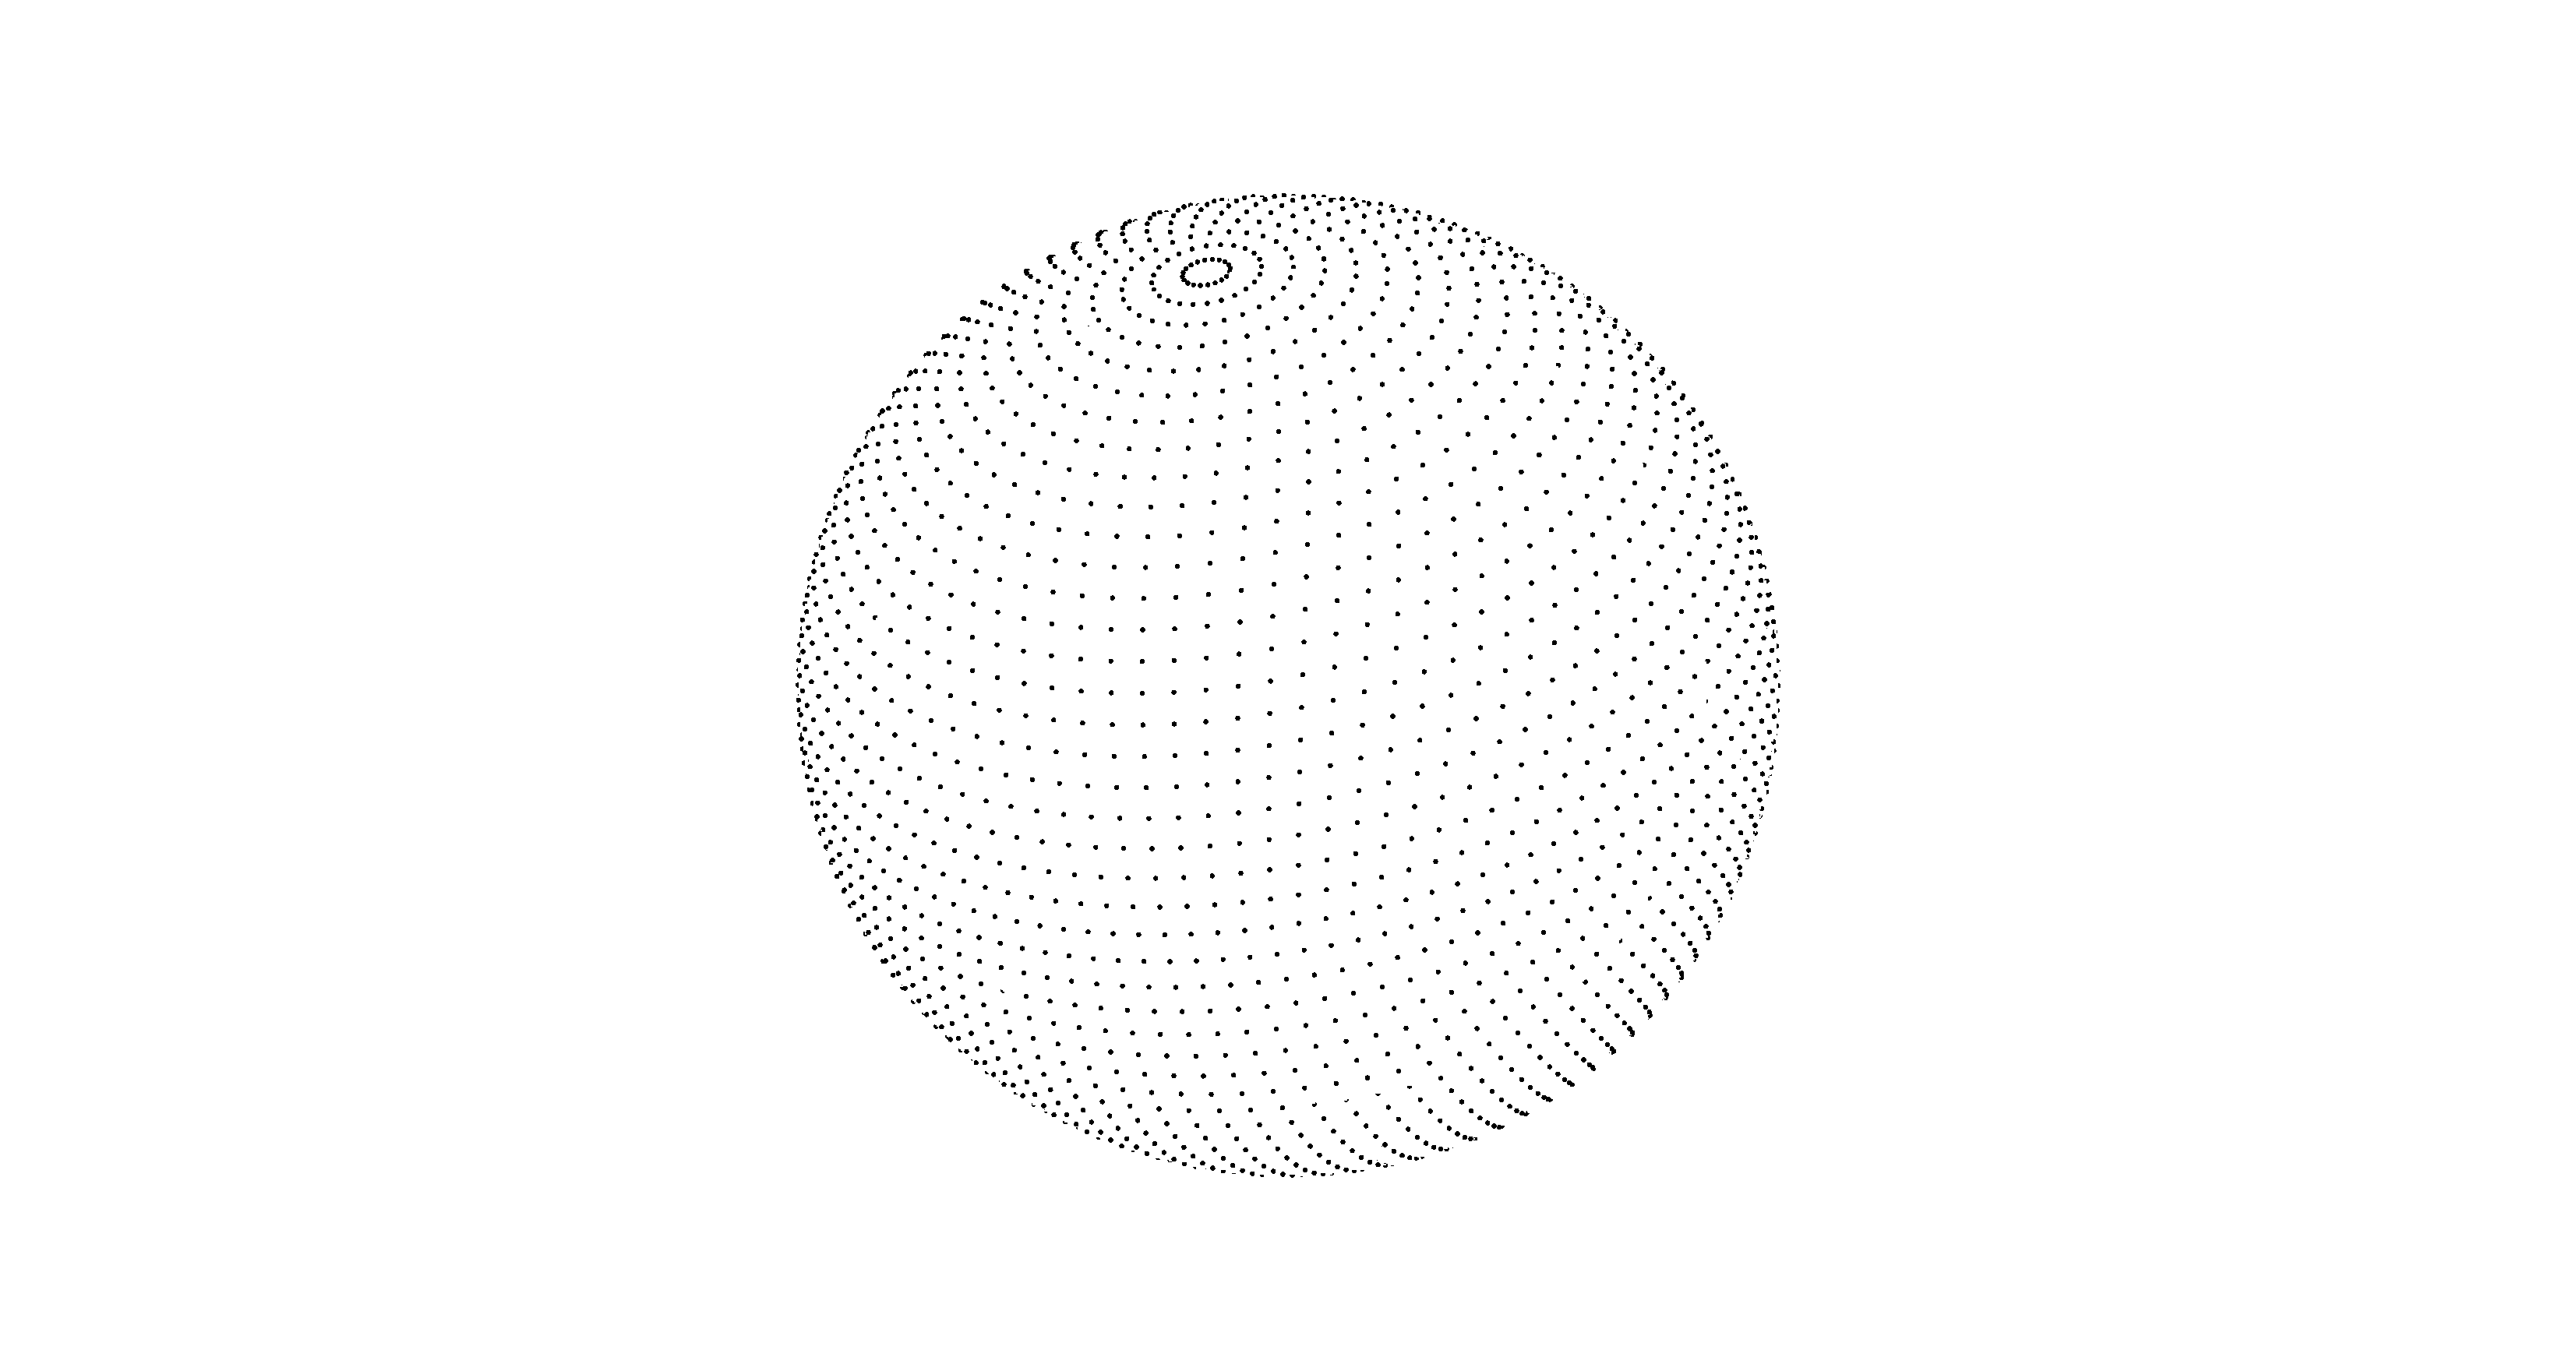
\includegraphics[width=5cm]{octahedral_gauss_nodes}
 \end{subfigure}%
\begin{subfigure}{.4\textwidth}
  \centering
  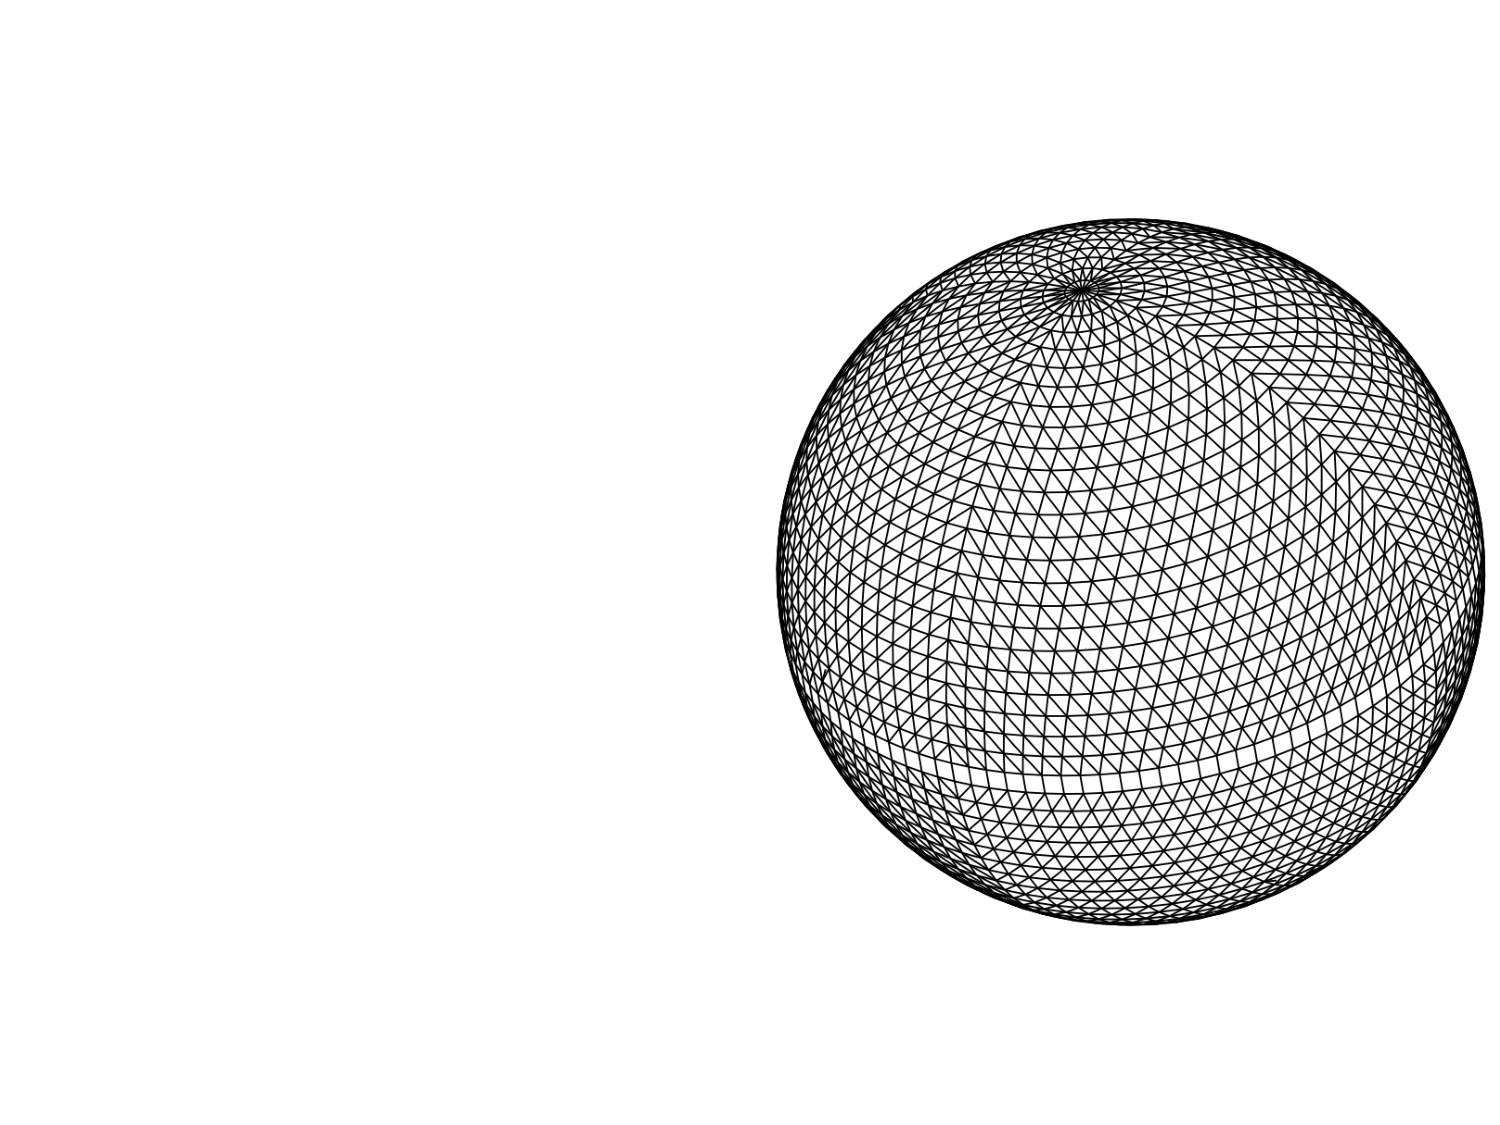
\includegraphics[width=4.7cm]{octahedral_RGG_white}
 \end{subfigure}
\caption{Locations of the octahedral reduced Gaussian grid nodes (left), and the edges of the primary mesh 
connecting the nodes as applied with the finite-volume discretisation in FVM (right). A coarse grid with only
24 latitudes between pole and equator is used for illustration. The dual mesh resolution of the octahedral
reduced Gaussian grid is about a factor 2 finer at the poles than the equator; see \cite{smolarkiewiczetalJCP2016}.}
\label{fig:octahedralgrid}
\end{figure}



%octahedral_RGG_white.pdf


%Fig.~\ref{fig:octahedralgridFVM} 


%%%%%%%%%%%%%%%%%%%%%%%%%%%%%%%%%%%%%%%%%%%%%%%%%%%%%%%%%%%%%

\section{Equation Sets} \label{sec:EquationSets}

{\color{red}[ALL] Include the continuous equation set that you use for your model here.}

\subsection{FVM} \label{sec:FVMEquations}

The fully compressible Euler equations solved in FVM are given as
\begin{subequations} \label{fvm:compressible}
\begin{align}
 & \pdiff{\mathcal{G}\rho_d}{t} + \nabla \cdot \left(\mathbf{v} \mathcal{G} \rho_d\right) = 0~,
\label{fvm:mass}  \\
& \pdiff{\mathcal{G} \rho_d \mathbf{u}}{t} + \nabla \cdot \left(\mathbf{v} \mathcal{G} \rho_d \mathbf{u} \right) = 
\mathcal{G}\rho_d\left( - \Theta \mathbf{\widetilde{G}} \nabla \phi' - \frac{ \mathbf{g}}{\theta_{a}} \left(\theta'+\theta_a (\epsilon q'_v - q_c - q_r) \right)
- \mathbf{f} \times \left( \mathbf{u} - \frac{\theta}{\theta_a} \mathbf{u}_{a} \right) 
+ \mathbf{M} \right)~,
\label{fvm:momentum} \\
%- \frac{L}{c_p \pi} & \Big( \frac{\Delta q_{vs}}{\Delta t} & + E_r  \Big)
& \pdiff{\mathcal{G}\rho_d \theta'}{t} + \nabla \cdot \left(\mathbf{v}\mathcal{G}\rho_d\,\theta' \right) = 
\mathcal{G}\rho_d\left(-\mathbf{\widetilde{G}}^{T}\mathbf{u} \cdot \nabla \theta_{a}
- \frac{L}{c_p \pi} \left( \frac{\Delta q_{vs}}{\Delta t}  + E_r  \right) %\left(C_d + E_p\right) 
+  \mathcal{H} \right)~,
\label{fvm:thermodynamic} \\
& \phi' = c_{p} \theta_{0} \left[\left( \frac{R_{d}}{p_{0}} \rho_d \theta (1+q_v/\varepsilon) \right)^{R_{d}/c_{v}} - \pi_{a} \right]~,
\label{fvm:gaslaw}
\end{align}
\end{subequations}
which describe the conservation laws of dry mass \eqref{fvm:mass}, momentum \eqref{fvm:momentum},
and dry entropy \eqref{fvm:thermodynamic}.
Dependent variables in \eqref{fvm:compressible} are dry density $\rho_d$, three-dimensional 
physical velocity vector $\mathbf{u}$, potential temperature perturbation $\theta'$, and Exner 
pressure perturbation $\pi'$, 
with the thermodynamic variables related by the gas law 
\eqref{fvm:gaslaw}~\footnote{Note that $\phi'$ represents a normalised Exner pressure perturbation.}.
Mixing ratios of water vapor, cloud condensate, and rain are denoted as $q_v$, $q_c$, and $q_r$,
respectively. All primed variables correspond to deviations from an ambient state (denoted by
subscript "a")  that satisfies 
a balanced subset of \eqref{fvm:compressible}, thus $\psi'=\psi-\psi_a$, where $\psi = u,v,w,\theta,..$~;
see \cite{prusa2008} and \cite{smolarkiewiczJCP2014}. 
The subscript "0" appearing with $\theta_0$ refers to a constant reference value. 
Symbols appearing on the rhs of the momentum equation \eqref{fvm:momentum}  are the
coefficient 
\begin{equation}
\Theta := \frac{\theta\,(1+q_v/\varepsilon)}{\theta_0\,(1+q_t)} %\equiv \frac{\theta_d}{\theta_0}~,
\end{equation}
in front of the pressure gradient term with $\Theta/\theta_0$ the density potential temperature,
the gravity vector $\mathbf{g} \equiv (0,0,-g)$~\footnote{In the shallow- versus deep-atmosphere 
form of the governing equations,  gravity is constant $g \equiv g_c$ or varies with height as 
$g = g_c\,(a/r)^2$, respectively.}, the Coriolis parameter $\mathbf{f}$, and  
$\epsilon=1/\varepsilon-1$ with $\varepsilon = R_d/R_v$. % and $\Upsilon_{C} := {\theta}/{\theta_a}$.
The governing equations \eqref{fvm:compressible} are formulated with respect to a geospherical 
coordinate system and a generalised height-based terrain-following vertical coordinate~\footnote{For
simplicity, the vertical coordinate is assumed to be time-independent in the current presentation.}.
Associated symbols are the Jacobian of the metric tensor $\mathcal{G}$, a matrix of metric coefficients
$\widetilde{\mathbf{G}}$, its transpose $\widetilde{\mathbf{G}}^{T}$, 
and the transformation of the physical to the contravariant velocity 
$\mathbf{v} = \mathbf{\widetilde{G}}^{T}\mathbf{u}$; see \cite{prusa2003} and \cite{kuehnleinJCP2012} for discussion.
%(see \eqref{prusa2003,kuehnleinJCP2012} for discussion). 
The symbol $\mathbf{M}$ in \eqref{fvm:momentum} subsumes metric forces due to the curvature
of the sphere \citep[][]{smolarkiewiczetalJCP2016} and momentum dissipation, whereas $\mathcal{H}$ 
in \eqref{fvm:thermodynamic} represents the diffusion of heat. 

%$\mathbf{M}$ and $\mathcal{H}$ subsume various rhs forcings to the
%momentum \eqref{fvm:momentum} and thermodynamic \eqref{fvm:thermodynamic} equations.




\subsection{Tempest} \label{sec:TempestEquations}

The continuity, momentum and thermodynamic equations can be written as:
\begin{align}
\pdiff{\rho}{t} &= - \nabla \cdot (\rho \vb{u}), \\
\pdiff{\vb{u}}{t} &= - \nabla (K + \Phi) - \theta \nabla \Pi + \vg{\eta} \times \vb{u}, \\
\pdiff{\theta_v}{t} &= - \vb{u} \cdot \nabla \theta_v,
\end{align} in terms of Kinetic energy $K = \vb{u} \cdot \vb{u}$, geopotential $\Phi = g_c z$ and absolute vorticity $\vg{\eta} = \vg{\zeta} + \vg{\Omega}$, which consists of relative vorticity $\vg{\zeta} = \nabla \times \vb{u}$ and planetary vorticity $\vg{\Omega}$.  The Exner pressure is related to the prognosed density and potential temperature via
\begin{equation} \label{eq:BaseNonhydrostaticEOS}
\Pi = c_p \left( \frac{p_0}{p} \right)^{R_d/c_p} = c_p \left( \frac{R_d \rho \theta_v}{p_0} \right)^{R_d/c_v}.
\end{equation}

\subsection{Tracer transport}

\noindent Lagrangian form:
\begin{align}
\diff{q}{t} &= 0.
\end{align}

\noindent Non-conservative Eulerian form:
\begin{align}
\pdiff{q}{t} &= - \vb{u} \cdot \nabla q.
\end{align}

\noindent Flux form:
\begin{align}
\pdiff{}{t} (\rho q) &= - \nabla \cdot (\rho q \vb{u}).
\end{align}


\subsection{Height-based coordinates}

{\color{blue}Define Unstaggered, Lorenz and Charney-Phillips staggering here}

\subsection{Mass-based coordinates}

%%%%%%%%%%%%%%%%%%%%%%%%%%%%%%%%%%%%%%%%%%%%%%%%%%%%%%%%%%%%%

\section{Diffusion and Stabilization} \label{sec:DiffusionStabilization}

{\color{red}[ALL] Include explicit diffusion and stabilization techniques that you have applied in the dynamical core here.}

\subsection{Scalar viscosity}

\noindent Scalar viscosity (direct):
\begin{align} \label{eq:scalar_viscosity_direct}
\diff{s}{t} &= \ldots + \nu \nabla \cdot \nabla s.
\end{align}

\noindent Scalar viscosity (conservative):
\begin{align} \label{eq:scalar_viscosity_conservative}
\diff{}{t} (\rho q) &= \ldots + \nu \nabla \cdot ( \rho \nabla q ).
\end{align}

\subsection{Smagorinsky eddy viscosity}

\subsection{Vector viscosity, divergence and vorticity damping}

\noindent Vector viscosity:
\begin{align} \label{eq:vector_viscosity}
\diff{\vb{u}}{t} &= \ldots + \nu \nabla^2 \vb{u}
\end{align}

\noindent Divergence damping:
\begin{align} \label{eq:divergence_damping}
\diff{\vb{u}}{t} &= \ldots + \nu_{div} \nabla (\nabla \cdot \vb{u})
\end{align}

\noindent Vorticity damping:
\begin{align} \label{eq:vorticity_damping}
\diff{\vb{u}}{t} &= \ldots + \nu_{vort} \nabla \times (\nabla \times \vb{u})
\end{align}

\subsection{Hyperviscosity} \label{sec:Diffusion_Hyperviscosity}

{\color{blue}Repeated application of the scalar and vector viscosity operators}

%%%%%%%%%%%%%%%%%%%%%%%%%%%%%%%%%%%%%%%%%%%%%%%%%%%%%%%%%%%%%

\section{Filters and Fixers} \label{sec:FiltersFixers}

{\color{red}[ALL] Include explicit filters and fixers that you have utilized in the dynamical core here.}

\subsection{Mass borrowing (positive definite preservation)}

\subsection{Mass fixers}

\subsection{Energy fixers}

%%%%%%%%%%%%%%%%%%%%%%%%%%%%%%%%%%%%%%%%%%%%%%%%%%%%%%%%%%%%%

\section{Temporal Discretizations} \label{sec:TemporalDiscretizations}

{\color{red}[ALL] Describe the time-stepping scheme / temporal discretization employed by your dynamical core here.}

\subsection{Runge-Kutta}

\subsubsection{Ullrich-Kinnmark-Gray 5 step 3rd order scheme} \label{sec:UKG53Scheme}

Explicit terms are evolved using a Runge-Kutta method which supports a large stability bound for spatial discretizations with purely imaginary eigenvalues. This particular scheme is based on \cite{kinnmark1984onestepA, kinnmark1984onestepB} and takes the form
\begin{align}
\psi^{(1)} &= \psi^{(0)} + \tfrac{\Delta t}{5} f(\psi^{(0)}), \nonumber \\
\psi^{(2)} &= \psi^{(0)} + \tfrac{\Delta t}{5} f(\psi^{(1)}), \nonumber \\
\psi^{(3)} &= \psi^{(0)} + \tfrac{\Delta t}{3} f(\psi^{(2)}), \\
\psi^{(4)} &= \psi^{(0)} + \tfrac{2 \Delta t}{3} f(\psi^{(3)}), \nonumber \\
\psi^{(5)} &= -\tfrac{1}{4} \psi^{(0)} + \tfrac{5}{4} \psi^{(1)} + \tfrac{3 \Delta t}{4} f(\psi^{(4)}). \nonumber
\end{align}

\subsection{Semi-implicit time integration of the fully compressible Euler equations in FVM}

In the following we provide an outline of the semi-implicit time stepping scheme for the fully 
compressible Euler equations in FVM (Section~\ref{sec:FVM}). 
A comprehensive discussion of the integration scheme can be found in \cite{smolarkiewiczJCP2014,smolarkiewiczetalJCP2016} 
for dry dynamics; and in \cite{kurowskiJAS2014} and \cite{smolarkiewiczetalMWR2017} for extensions to 
moist dynamics. 
The generic two-time-level second-order template algorithm employed in the integration is given as
\begin{equation}
\psi_{\mbf{i}}^{n+1}= \mathcal{A}_{\mbf{i}}(\widetilde{\psi}^{n},\mathbf{V}^{n+1/2}, (\mathcal{G}\rho_d)^{n}, (\mathcal{G}\rho_d)^{n+1})
+0.5\,\Delta t\,R^{\psi}|_{\mbf{i}}^{\scs n+1}~,
\hspace{1em} \widetilde{\psi}^{n}\,\equiv\,\psi^n+0.5\,\Delta t\,R^{\psi}|^{\scs n}~.
\label{fvm:solscalar}
\end{equation}
In \eqref{fvm:solscalar}, $\psi$ represents the solution variable, $R^{\psi}$ is the respective rhs,
and $\mathcal{A}$ symbolises an advective transport operator assumed here to be the non-oscillatory 
finite-volume MPDATA (Multidimensional Positive Definite Advection Transport Algorithm) scheme 
\citep{smolarkiewiczszmelter2005,kuehnleinJCP2016}~\footnote{Furthermore, 
in \eqref{fvm:solscalar} the vector index $\mathbf{i}$ denotes the spatial position 
on the computational grid, $\Delta t$ is the time step size between levels $n$ and $n+1$.}. 

The integration of the system \eqref{fvm:compressible} can basically be divided into three steps. First, the homogenous
mass continuity equation is integrated with $\psi \equiv \rho_d$, $\mathbf{V} \equiv \mathbf{v}\mathcal{G} $,
and $R^{\rho_d} \equiv 0$ in \eqref{fvm:solscalar}. Second, the thermodynamic \eqref{fvm:thermodynamic}, 
momentum \eqref{fvm:momentum}, and moisture equations enter
\eqref{fvm:solscalar} with $\psi = u, v, w, \theta',...$, $\mathbf{V} \equiv \mathbf{v}\mathcal{G}\rho_d$, and the rhs $R^{\psi}$ 
which is generally depending on all prognostic variables. A high degree of implicitness in the representation of the rhs forcings
is achieved by inverting the overall discrete system \eqref{fvm:solscalar} to obtain closed-form expressions for the
velocity updates -- the procedure is facilitated by the co-located arrangement of variables on the computational mesh. %indicated by the spatial mesh vector index..
Retained on the rhs of the derived closed-form velocity expressions is the pressure gradient term. 
The third step in the solution procedure is to formulate an implicit boundary value problem for the pressure variable $\phi'$ using 
an evolutionary form of the equation of state \eqref{fvm:gaslaw}. An $\mathcal{O}(\Delta t^2)$ integration of this 
equation with a Euler backward template algorithm in the spirit of \eqref{fvm:solscalar} leads a Helmholtz equation. 
The associated 3D elliptic boundary value problem is solved iteratively using a bespoke preconditioned Generalised Conjugate 
Residual approach \citep{smolarkiewiczECMWF2004,smolarkiewiczAG2011}.
Nonlinearities in $R^{\psi}$ and the solution-dependent coefficients of the Helmholtz problem are lagged behind and 
executed in an outer iteration.
 
%The overall integration scheme is 3d implicit with respect to the fast acoustic and buoyant as well as 
%slow rotational modes.


%The integration scheme of FVM approximates the generic conservation law
%\begin{equation}
%\frac{\partial \rho\mathcal{G}\Psi}{\partial t} + \nabla \cdot \left(\rho\mathcal{G}\mathbf{v}  \Psi \right) = \rho\mathcal{G}R^{\Psi}~, %\hspace{1em} 
%\label{scalar}
%\end{equation}
%which represents any of the governing equations \eqref{fvm:mass}-\eqref{fvm:thermodynamic}
%(i.e.~$\Psi = 1 , u, v, w, \theta'$,  as well as corresponding rhs $R^{\Psi}$), by the 
%second-order template algorithm
%\begin{equation}
%\Psi_{\mbf{i}}^{n+1}= \mathcal{A}_{\mbf{i}}(\widetilde{\Psi}^{n},(\rho \mathcal{G} v^{\perp})^{n+1/2}, (\rho\mathcal{G})^{n}, (\rho\mathcal{G})^{n+1})
%+0.5\,\delta t\,R^{\Psi}|_{\mbf{i}}^{\scs n+1}~,
%\hspace{1em} \widetilde{\Psi}^{n}\,\equiv\,\Psi^n+0.5\,\delta t\,R^{\Psi}|^{\scs n}~,
%%\hspace{1em} \widetilde{\psi}^{n}$\,$\equiv$\,$\psi^n+0.5\,\delta\ol{t}\,R^{\psi}|^{\scs n}~,
%\label{solscalar}
%\end{equation}
%where $\mathcal{A}$ is a shorthand for the advective transport operator MPDATA. The index $\mathbf{i}$ 
%denotes the spatial position on the computational grid, $\delta t$ is the time step size between levels $n$
%and $n+1$, 



%%%%%%%%%%%%%%%%%%%%%%%%%%%%%%%%%%%%%%%%%%%%%%%%%%%%%%%%%%%%%

\section{Dynamical Cores}

{\color{red}In this section provide a short description (approximately 0.5 pages) of the dynamical core, focusing on unique features or design specifications.  Do not include information on the physical parameterizations used by the modeling system.  Make reference to the model grid employed from section \ref{sec:ModelGrids}, the specific equation set being discretized by the model in section \ref{sec:EquationSets}, explicit numerical techniques for diffusion and stabilization in section \ref{sec:DiffusionStabilization}, filters and fixers in section \ref{sec:FiltersFixers} and the temporal discretization in section \ref{sec:TemporalDiscretizations}.}

\subsection{Tempest}

{\color{red}[ULLRICH]}

The Tempest model \citep{ullrich2014global, guerra2016high} uses a horizontal spectral element discretization and vertical staggered nodal finite element method based on the cubed-sphere grid with terrain-following height-based coordinate.  The standard Eulerian equations are employed with moist density $\rho$, thermodynamic closure $\theta_v$ and tracer density $\rho q$.  These continuous equations are given in section \ref{sec:TempestEquations}.  The implementation includes both fully explicit time integration, using the UKG53 scheme described in section \ref{sec:UKG53Scheme}, and implicit-explicit options, where horizontal terms are explicitly discretized and vertical terms are treated implicitly.  Scalar hyperviscosity is employed for $\rho$, $\theta$ and tracer variables via repeated application of (\ref{eq:scalar_viscosity_direct}).  Vector hyperviscosity is also applied by decomposing the horizontal vector Laplacian into divergence damping (\ref{eq:divergence_damping}) and vorticity damping (\ref{eq:vorticity_damping}) terms.  Both viscosity operations are applied after the completion of all Runge-Kutta sub-cycles.

\subsection{High-Order Method Modeling Environment (HOMME)}

{\color{red}[HALL]}

\subsection{Model for Prediction Across Scales (MPAS)}

{\color{red}[SKAMAROCK]}

\subsection{Colorado State University Model (CSU)}

{\color{red}[RANDALL]}

\subsection{Geophysical Fluid Dynamics Laboratory FV Cubed (GFDL-FV3)}

{\color{red}[HARRIS]}

\subsection{Chombo}

{\color{red}[JOHANSEN]}

\subsection{Naval Research Laboratory NEPTUNE Model}

{\color{red}[VINER, REINECKE]}

\subsection{Global Environmental Multiscale (GEM) Model}

{\color{red}[LEE]}

\subsection{Ocean-Land-Atmosphere Model (OLAM)}

{\color{red}[WALKO]}

\subsection{DYNAMICO}

{\color{red}[DUBOS]}

\subsection{Finite-volume module of the Integrated Forecasting System}
\label{sec:FVM}

%{\color{red}[KUEHNLEIN]}

The finite-volume module (FVM) of the Integrated Forecasting System (IFS) is developed at 
ECMWF \citep{smolarkiewiczetalJCP2016}. FVM solves the fully compressible Euler 
equations in geospherical coordinates. Both deep-atmosphere and shallow-atmosphere equations 
are available by means of simple switches. The formulation incorporates 
a generalised, optionally time-dependent, terrain-following vertical coordinate based on height. 
A centred two-time-level semi-implicit integration scheme is employed with 3D implicit treatment 
of acoustic, buoyant, and rotational modes \citep{smolarkiewiczJCP2014}. The associated 3D 
Helmholtz problem is solved iteratively using a bespoke preconditioned Generalised 
Conjugate Residual approach. 
The integration procedure uses the multidimensional flux-form Eulerian non-oscillatory MPDATA 
advection scheme \citep{smolarkiewiczszmelter2005,kuehnleinJCP2016}. 
The horizontal spatial discretisation is fully unstructured finite-volume using the 
median-dual approach. This is combined with a structured-grid finite-difference approach in the 
vertical direction; see \cite{smolarkiewiczetalJCP2016} for an exposition. 
In both the horizontal and the vertical discretisation, all prognostic variables are 
co-located. The median-dual finite-volume mesh in the horizontal is developed about the points/nodes 
of the octahedral reduced Gaussian grid (Section~\ref{subsection:octahedralreducedgaussiangrid}). The octahedral 
reduced Gaussian grid is also employed in the spectral dynamical core of the current operational 
IFS at ECMWF, which facilitates interoperability of the two formulations. However, we note that FVM is 
not restricted to this grid and offers capabilities towards a broad classes of meshes including adaptivity. 


No explicit diffusion is applied in FVM for DCMIP, apart from the momentum dissipation and scalar 
diffusion required for some of the test cases, which is the vertical dissipation/diffusion in the planetary
boundary layer parametrisation and the constant-coefficient second-order dissipation/diffusion in 
the supercell test. An absorbing layer in the first latitude ring around the poles is optionally used in 
the form of a Rayleigh-type forcing to the prognostic variables. The dynamics time step is adapted 
at every time step according to a given maximum advective CFL number (typically somewhat smaller 
than 1). The physics time step is identical to the dynamics time step. 
%The first row of the table below refers to the size of the octahedral reduced Gaussian grid, where 
%the number following "O" (for octahedral) denotes the number of latitudes between pole and equator.


%Neither explicit diffusion/filters nor decentering of the time-stepping scheme is applied in DCMIP, 
%No explicit diffusion is applied in FVM in DCMIP, apart from the explicit momentum dissipation and 
%scalar diffusion required for some of the test cases.  FVM uses adaptive time stepping for optimal
%efficiency and accuracy. 
 
%FVM employs distributed- and shared-memory parallelisation using the MPI and OpenMP standards, 
%respectively. %The underlying distributed-memory data structures in FVM are provided by the Atlas 
%framework developed at ECMWF. 

\subsection{Icosahedral Non-hydrostatic (ICON) Model}

{\color{red}[GIORGETTA]}

\subsection{Nonhydrostatic ICosahedral Atmospheric Model (NICAM) Model}

{\color{red}[MIURA]}

%%%%%%%%%%%%%%%%%%%%%%%%%%%%%%%%%%%%%%%%%%%%%%%%%%%%%%%%%%%%%

\section{Idealized Physical Parameterizations}

\subsection{Kessler Physics} \label{sec:KesslerPhysics}

The cloud microphysics update according to the following equation set:
\begin{alignat}{5}
\frac{\Delta \theta}{\Delta t} = & - \frac{L}{c_p \pi} & \Big( \frac{\Delta q_{vs}}{\Delta t} & + E_r  \Big) & \\
\frac{\Delta q_v}{\Delta t} = & & \frac{\Delta q_{vs}}{\Delta t} & + E_r \\
\frac{\Delta q_c}{\Delta t} = & & - \frac{\Delta q_{vs}}{\Delta t} & & - A_r & - C_r \\
\frac{\Delta q_r}{\Delta t} = & & & - E_r & + A_r & + C_r & - V_r \pdiff{q_r}{z},
\end{alignat} where $L$ is the latent heat of condensation, $A_r$ is the autoconversion rate of cloud water to rain water, $C_r$ is the collection rate of rain water, $E_r$ is the rain water evaporation rate, and $V_r$ is the rain water terminal velocity.

The pressure follows from the equation of state
\begin{equation}
p=\rho R_dT(1+0.61q_v)
\end{equation} with $p$ the pressure, $\rho$ the density of moist air, $R_d$ the gas constant for dry air, $T$ the temperature and $q_v$ the mixing ratio of water vapor. The equation is rewritten as a nondimensional pressure $\Pi$ equation.
\begin{equation}
\pi = \left(\frac{p}{p_0}\right)^{\frac{R_dT}{cp}}
\end{equation}

To determine the saturation vapor mixing ratio the Teten's formula is used,
\begin{equation}
q_{vs}(p,T) = \left( \frac{380.0}{p} \right) \exp\left(17.27 \times \frac{T-273.0}{T-36.0}\right)
\end {equation}

The autoconvection rate ($A_r$) and collection rate ($C_r$) follow Kessler parametrization and are defined by:
\begin{align}
A_r &= k_1(q_c-a) \\
C_r &= k_2q_cq_r^{0.875}
\end{align} With $k_1=0.001 \text{s}^{-1}$, $a=0.001 \text{g}.\text{g}^{-1}$ and $k_2=2.2 \text{s}^{-1}$ 

Deriving from \cite{klemp1978simulation} description of cloud water,rain water and water vapor mixing ratios. they are define as followed:
\begin{equation}
q_c^{n+1}=\mbox{max}(q_c^r-\Delta q_r,0)
\end{equation}
\begin{equation}
q_r^{n+1}=\mbox{max}(q_r^r-\Delta q_r+S,0)
\end{equation} where $S$ is the sedimentation term and $\Delta q_r$ is defined as
\begin{equation}
\Delta q_r=q_c^n-\frac{q_c^n-\Delta \text{t}\ \mbox{max}(A_r,0)}{1+\Delta \text{t} C_r}
\end{equation}

The Rain evaporation equation is defined similarly to \cite{ogura1971numerical} description:
\begin{equation}
E_r=\frac{1}{\rho}\frac{\left(1-\frac{q_v}{q_{vs}}\right)C(\rho q_r)^{0.525}}{5.4\times10^5+\frac{2.55\times10^6}{pq_{vs}}}
\end{equation}  With ventilation factor C define as 
\begin{equation}
C_r=1.6+124.9(\rho q_r)^{0.2046}
\label{venti}
\end{equation}

The liquid water terminal velocity is similar to \cite{soong1973comparison} description with a mean density adjustment as suggested by \cite{kessler1969distribution}:
\begin{equation}
V_r = 36349(\rho q_r)^{0.1346}\left(\frac{\rho}{\rho_0}\right)^{-\frac{1}{2}}
\end{equation}

%%%%%%%%%%%%%%%%%%%%%%%%%%%%%%%%%%%%%%%%%%%%%%%%%%%%%%%%%%%%%

\subsection{Simplified Mixing in the Planetary Boundary Layer} \label{sec:PlanetaryBoundaryLayer}

The forcing by the planetary boundary layer is described in \cite{reed2012idealized} and is partly reproduced here.  To parameterize the surface fluxes that impact the zonal velocity $u$, the meridional velocity $v$ and moisture $q$ we start with the time rate of change equations
\begin{eqnarray}
\frac{\partial u}{\partial t} &=& - \frac{1}{\rho} \frac{\partial \rho \ \overline{w'u'}}{\partial z} \label{eqturb}  \\
\frac{\partial v}{\partial t} &=& - \frac{1}{\rho} \frac{\partial \rho \ \overline{w'v'}}{\partial z}  \label{eqturb_v} \\
\frac{\partial q}{\partial t} &=& - \frac{1}{\rho} \frac{\partial \rho \ \overline{w'q'}}{\partial z}.  \label{eqturb_last}
\end{eqnarray}  Potential temperature, as opposed to temperature, is used in the boundary layer parameterization because the vertical profile of the potential temperature is a suitable indicator of static stability.  This adds the time rate of change equation
\begin{eqnarray}
\frac{\partial \Theta}{\partial t} &=& - \frac{1}{\rho} \frac{\partial \rho \ \overline{w'\Theta'}}{\partial z}.
\end{eqnarray}  Here $u'$, $v'$, $w'$, $\Theta'$ and $q'$ symbolize the deviations of the zonal velocity, meridional velocity, vertical velocity, potential temperature and specific humidity from their averages, respectively. The average is indicated by an overbar.  Note, assuming pressure is held constant (which is a common assumption in physical parameterizations), the potential temperature time tendency can be converted back to a temperature tendency of the following form
\begin{eqnarray}
\frac{\partial T}{\partial t} &=& - \frac{1}{\rho} \left (\frac{p}{p_0} \right )^{\kappa} \frac{\partial \rho \ \overline{w'\Theta'}}{\partial z}.
\end{eqnarray}
with the reference pressure $p_0 = 1000$ hPa.

The turbulent mixing is characterized by a constant vertical eddy diffusivity to represent Ekman-like profiles of boundary layers
\begin{eqnarray}\label{ktheory}
\overline{w'u'} = -K_m \frac{\partial u}{\partial z} \\
\overline{w'v'} = -K_m \frac{\partial v}{\partial z} \\
\overline{w'\Theta'} = -K_E \frac{\partial \Theta}{\partial z} \\
\overline{w'q'} = -K_E \frac{\partial q}{\partial z}. 
\end{eqnarray}
Here, $K_m$ is the eddy diffusivity coefficient for momentum and $K_E$ is the eddy diffusivity coefficient for energy and set equal to that for water vapor. In order to calculate the eddy diffusivity coefficients, the eddy diffusivity is matched to that for the surface flux calculated in Appendix~\ref{sec:OceanSurfaceFluxes} at the lowermost model level.  To allow for a smooth transition above the boundary layer ($p_{top} = 850$ hPa)  the diffusivity coefficients for momentum taper to zero as
\begin{equation} \label{Kmtaper}
\begin{array}{ll}
K_m = C_d \vert \vec{v}_{a} \vert z_a & \mbox{for} \; p > p_{top} \\
K_m = C_d \vert \vec{v}_{a} \vert z_a \exp \left ( -\left [ \frac{p_{top} - p}{p_{strato}} \right ]^2 \right ) & \mbox{for} \; p \leq p_{top}.
\end{array}
\end{equation}
Here the constant $p_{strato}$ determines the rate of decrease and is set to 100 hPa. $K_E$ is defined by
\begin{equation}
\begin{array}{ll}\label{KEtaper}
K_E = C_E \vert \vec{v}_{a} \vert z_a & \mbox{for} \; p > p_{top} \\
K_E = C_E \vert \vec{v}_{a} \vert z_a \exp \left ( -\left [ \frac{p_{top} - p}{p_{strato}} \right ]^2 \right ) & \mbox{for} \; p \leq p_{top}.
\end{array}
\end{equation}
We suggest implementing the boundary layer scheme with an implicit temporal discretization to avoid numerical instabilities. The details of this discretization are somewhat complicated, and so we refer to implementation details in Appendix D of \cite{reed2012idealized}. In addition, we supply the DCMIP modeling groups with the complete ``simple-physics'' package as used in the model CAM which can serve as a template routine.

\conclusions  %% \conclusions[modified heading if necessary]
TEXT




%\appendix
%\section{}    %% Appendix A

%\subsection{}                               %% Appendix A1, A2, etc.


\authorcontribution{TEXT}

\begin{acknowledgements}
{\color{blue}[Include a complete list of DCMIP2016 student participants here along with sponsors]}
\end{acknowledgements}


%% REFERENCES

%% Since the Copernicus LaTeX package includes the TeX style file copernicus.bst,
%% authors experienced with BibTeX only have to include the following two lines:
%%
\bibliographystyle{copernicus}
\bibliography{DCMIP2016,../../bib/fvm}
%\bibliography{fvm}
%%
%% URLs and DOIs can be entered in your BibTeX file as:
%%
%% URL = {http://www.xyz.org/~jones/idx_g.htm}
%% DOI = {10.5194/xyz}


%% LITERATURE CITATIONS
%%
%% command                        & example result
%% \citet{jones90}|               & Jones et al. (1990)
%% \citep{jones90}|               & (Jones et al., 1990)
%% \citep{jones90,jones93}|       & (Jones et al., 1990, 1993)
%% \citep[p.~32]{jones90}|        & (Jones et al., 1990, p.~32)
%% \citep[e.g.,][]{jones90}|      & (e.g., Jones et al., 1990)
%% \citep[e.g.,][p.~32]{jones90}| & (e.g., Jones et al., 1990, p.~32)
%% \citeauthor{jones90}|          & Jones et al.
%% \citeyear{jones90}|            & 1990



%% FIGURES

%% ONE-COLUMN FIGURES

%%f
%\begin{figure}[t]
%\includegraphics[width=8.3cm]{FILE NAME}
%\caption{TEXT}
%\end{figure}
%
%%% TWO-COLUMN FIGURES
%
%%f
%\begin{figure*}[t]
%\includegraphics[width=12cm]{FILE NAME}
%\caption{TEXT}
%\end{figure*}
%
%
%%% TABLES
%%%
%%% The different columns must be seperated with a & command and should
%%% end with \\ to identify the column brake.
%
%%% ONE-COLUMN TABLE
%
%%t
%\begin{table}[t]
%\caption{TEXT}
%\begin{tabular}{column = lcr}
%\tophline
%
%\middlehline
%
%\bottomhline
%\end{tabular}
%\belowtable{} % Table Footnotes
%\end{table}
%
%%% TWO-COLUMN TABLE
%
%%t
%\begin{table*}[t]
%\caption{TEXT}
%\begin{tabular}{column = lcr}
%\tophline
%
%\middlehline
%
%\bottomhline
%\end{tabular}
%\belowtable{} % Table Footnotes
%\end{table*}
%
%
%%% NUMBERING OF FIGURES AND TABLES
%%%
%%% If figures and tables must be numbered 1a, 1b, etc. the following command
%%% should be inserted before the begin{} command.
%
%\addtocounter{figure}{-1}\renewcommand{\thefigure}{\arabic{figure}a}
%
%
%%% MATHEMATICAL EXPRESSIONS
%
%%% All papers typeset by Copernicus Publications follow the math typesetting regulations
%%% given by the IUPAC Green Book (IUPAC: Quantities, Units and Symbols in Physical Chemistry,
%%% 2nd Edn., Blackwell Science, available at: http://old.iupac.org/publications/books/gbook/green_book_2ed.pdf, 1993).
%%%
%%% Physical quantities/variables are typeset in italic font (t for time, T for Temperature)
%%% Indices which are not defined are typeset in italic font (x, y, z, a, b, c)
%%% Items/objects which are defined are typeset in roman font (Car A, Car B)
%%% Descriptions/specifications which are defined by itself are typeset in roman font (abs, rel, ref, tot, net, ice)
%%% Abbreviations from 2 letters are typeset in roman font (RH, LAI)
%%% Vectors are identified in bold italic font using \vec{x}
%%% Matrices are identified in bold roman font
%%% Multiplication signs are typeset using the LaTeX commands \times (for vector products, grids, and exponential notations) or \cdot
%%% The character * should not be applied as mutliplication sign
%
%
%%% EQUATIONS
%
%%% Single-row equation
%
%\begin{equation}
%
%\end{equation}
%
%%% Multiline equation
%
%\begin{align}
%& 3 + 5 = 8\\
%& 3 + 5 = 8\\
%& 3 + 5 = 8
%\end{align}
%
%
%%% MATRICES
%
%\begin{matrix}
%x & y & z\\
%x & y & z\\
%x & y & z\\
%\end{matrix}
%
%
%%% ALGORITHM
%
%\begin{algorithm}
%\caption{�}
%\label{a1}
%\begin{algorithmic}
%�
%\end{algorithmic}
%\end{algorithm}
%
%
%%% CHEMICAL FORMULAS AND REACTIONS
%
%%% For formulas embedded in the text, please use \chem{}
%
%%% The reaction environment creates labels including the letter R, i.e. (R1), (R2), etc.
%
%\begin{reaction}
%%% \rightarrow should be used for normal (one-way) chemical reactions
%%% \rightleftharpoons should be used for equilibria
%%% \leftrightarrow should be used for resonance structures
%\end{reaction}
%
%
%%% PHYSICAL UNITS
%%%
%%% Please use \unit{} and apply the exponential notation


\end{document}
